\documentclass{article}
% translate with >> pdflatex -shell-escape <file>

% This file is used as unit test for pgfplots, copyright by Christian Feuersaenger.
% 
% See
%   http://pgfplots.sourceforge.net/pgfplots.pdf
% for pgfplots.
%
% Any required input files (for <plot table> or <plot file> or the table package) can be downloaded
% at
% http://www.ctan.org/tex-archive/graphics/pgf/contrib/pgfplots/doc/latex/
% and
% http://www.ctan.org/tex-archive/graphics/pgf/contrib/pgfplots/doc/latex/plotdata/

\usepackage{pgfplots}
\pgfplotsset{compat=1.3}

\pagestyle{empty}

\begin{document}

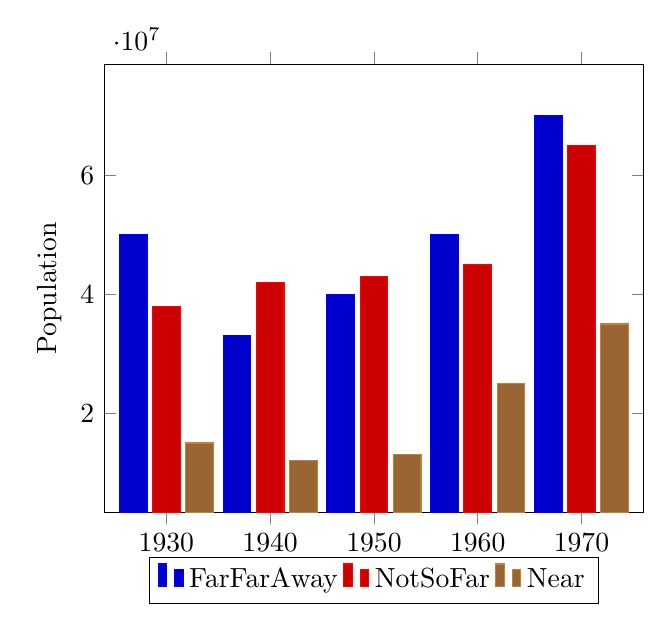
\begin{tikzpicture}
	\begin{axis}[
		%xmin=1925,xmax=1975,disabledatascaling=false,
		%xtick={1930,1940,1950,1960,1970},
		x tick label style={/pgf/number format/set thousands separator=},
		ylabel=Population,
		enlargelimits=0.15,
		legend style={at={(0.5,-0.1)},anchor=north,legend columns=-1},
		ybar,
	]
%\tracingmacros=2\tracingcommands=2
	\addplot[draw=blue,mark=none,fill=blue!80!black] 
		plot coordinates {(1930,50e6) (1940,33e6) (1950,40e6) (1960,50e6) (1970,70e6)};
	\addlegendentry{FarFarAway}

	\addplot[mark=none,red,fill=red!80!black] 
		plot coordinates {(1930,38e6) (1940,42e6) (1950,43e6) (1960,45e6) (1970,65e6)};
	\addlegendentry{NotSoFar}

	\addplot[mark=none,brown,fill=brown!80!black] 
		plot coordinates {(1930,15e6) (1940,12e6) (1950,13e6) (1960,25e6) (1970,35e6)};
	\addlegendentry{Near}
	\end{axis}
\end{tikzpicture}
\end{document}
